\documentclass[11pt,a4paper]{article}
% Shared article style for handouts.
\usepackage[fontset=none]{ctex}
\usepackage{fontspec}
\setmainfont{DejaVu Serif}
\setsansfont{DejaVu Sans}
\setmonofont{DejaVu Sans Mono}
\setCJKmainfont{Noto Serif CJK SC}[BoldFont={Noto Serif CJK SC Bold}]
\setCJKsansfont{Noto Sans CJK SC}[BoldFont={Noto Sans CJK SC Bold}]
\setCJKmonofont{Noto Sans Mono CJK SC}

\usepackage[margin=1in]{geometry}
\usepackage{graphicx}
\usepackage{enumitem}
\usepackage{amsmath,amssymb}
\usepackage{booktabs,array}
\usepackage{xcolor}
\usepackage{listings}
\usepackage{tcolorbox}
\tcbuselibrary{breakable}
\usepackage{hyperref}

\definecolor{hcPrimary}{RGB}{20,72,110}
\definecolor{hcTipBG}{RGB}{239,246,252}
\definecolor{hcTipFrame}{RGB}{80,126,160}
\definecolor{hcWarnBG}{RGB}{253,244,238}
\definecolor{hcWarnFrame}{RGB}{183,84,52}
\definecolor{hcCodeBG}{RGB}{247,248,250}
\definecolor{hcCodeFrame}{RGB}{208,214,220}

\hypersetup{colorlinks=true,linkcolor=hcPrimary,urlcolor=hcPrimary,citecolor=hcPrimary}
\setlist{nosep}

\newtcolorbox{tipbox}{
  colback=hcTipBG,
  colframe=hcTipFrame,
  title=提示,
  fonttitle=\bfseries,
  boxrule=0.6pt,
  breakable
}

\newtcolorbox{warnbox}{
  colback=hcWarnBG,
  colframe=hcWarnFrame,
  title=警告,
  fonttitle=\bfseries,
  boxrule=0.6pt,
  breakable
}

\lstset{
  basicstyle=\ttfamily\footnotesize,
  backgroundcolor=\color{hcCodeBG},
  frame=single,
  rulecolor=\color{hcCodeFrame},
  numbers=left,
  numberstyle=\tiny,
  breaklines=true,
  showstringspaces=false,
  tabsize=2
}


\title{第三章第一讲：数字抽象、CMOS 与组合逻辑基础}
\author{Digital Circuit Getting Started}
\date{\today}

\graphicspath{{figures/}}

\begin{document}
\maketitle

\section{本讲导读}

第三章不能被写成一份“逻辑门名词表”，因为那样会把最关键的问题遮掉：数字系统之所以能成立，并不是因为课本上先发明了 0 和 1，而是因为真实器件、真实电压范围、真实延迟和真实噪声，恰好允许我们在工程上建立一层足够稳定的数字抽象。本讲的任务，就是把这层抽象从物理世界里重新长出来。

在第一章里，我们已经知道数字抽象是管理复杂系统的基础；在第二章里，我们又先走通了最小工具闭环。但如果还不知道“逻辑从哪里来”，后面学到的布尔代数、RTL、综合与时序分析，很容易退化成一堆互不相连的技巧。本讲因此要沿着一条很明确的因果链推进：先看 MOS 管怎样提供受控导通路径，再看 CMOS 反相器怎样把这种器件行为组织成稳定的逻辑翻转，然后扩展到 NAND、NOR 与组合逻辑，最后用环形振荡器、竞争与冒险提醒自己，时间问题并不是后端才出现的附属细节。

这里有一个很重要的边界要先守住。本讲不是半导体器件课程的缩略版，也不是标准单元库或综合优化的预备课。我们不会推长沟道模型公式，不会系统展开版图工艺规则，也不会提前滑进 logic effort 和完整 STA。目标更朴素，也更基础：让读者第一次真正把“数字抽象的物理依据”“逻辑门的结构语义”“组合逻辑里的最小时序直觉”接到一起。

\section{Learning Objectives}

读完这一讲，你应当能够：

\begin{itemize}
  \item 理解数字抽象为什么成立，以及它至少依赖哪些工程前提。
  \item 用“栅控导通、上拉 / 下拉网络”的语言解释 NMOS、PMOS 与静态 CMOS 的最小工作方式。
  \item 说明 CMOS 反相器为什么是数字世界的最小完整基元，并能解释输入高低变化时的导通路径。
  \item 看懂电压传输特性（VTC）、噪声容限、充电 / 放电路径与短路电流这些概念在解释什么。
  \item 知道门延迟为什么不是静态常数，以及 fanout、负载和 transition 怎样进入延迟问题。
  \item 从晶体管网络的角度理解 NAND / NOR 的静态 CMOS 结构，并知道逻辑门最后会落成规则化的物理单元。
  \item 在真值表、布尔表达式与门级结构之间来回转换，并用半加器作为收束例子。
  \item 解释组合逻辑中的竞争与冒险为什么出现，以及为什么它们不能被简单视作“无害瞬态”。
\end{itemize}

\section{为什么这一讲值得学}

很多教材会把“数字电路”直接从逻辑门符号开始讲：与门、或门、非门、真值表、布尔公式，像搭积木一样一层层往上堆。这样的组织方式并不算错，但它有一个明显副作用：学生很容易误以为逻辑门是某种脱离物理世界独立存在的数学对象，仿佛先有布尔代数，后有电路去把它“实现”出来。真正的工程顺序恰好相反。先有能在真实电压和真实器件上稳定工作的一套结构，布尔语言才有机会成为一种可靠的抽象层。

这也是为什么本讲必须从器件开始，但又不能陷在器件细节里。只盯着公式推导，你会失去后面那条“从器件到逻辑门再到组合逻辑”的主线；只盯着门符号，你又会忘记这些门最后必须落成可制造、可复制、可级联的物理对象。教学上的困难，恰好在于要同时保住两件事：既让读者看到数字抽象是如何被物理世界托起来的，又不把第一讲写成半导体器件专论。

还有一个更隐蔽但更关键的理由。本讲虽然讲的是“组合逻辑”，却已经在为后面的时序问题埋下地基。反相器的充电 / 放电、负载变化带来的延迟拉长、环形振荡器对门延迟的敏感性、不同路径延迟导致的毛刺，这些现象都在提醒我们：时间问题并不是系统进入寄存器和时钟之后才突然出现，而是从第一个门电路开始就已经存在。下一讲讲 setup、hold、skew 和 metastability 时，这条线会继续被点亮。

\section{核心概念与对象}

\subsection{数字抽象为什么成立}

现实世界本质上是连续的。电路里的信号是随时间变化的电压和电流，器件有阈值、有噪声、有延迟，温度和工艺还会进一步扰动这些行为。如果一直停留在纯模拟视角来组织全部数字系统，复杂度会很快失控。数字抽象的价值，正在于它把这一团连续世界组织成一套离散规则：一段电压范围被当作逻辑 0，另一段电压范围被当作逻辑 1，中间模糊区尽量避免长期停留；组合逻辑在时钟周期内收敛，寄存器在离散时刻捕获状态。

但这套抽象不是天然成立的。它至少依赖三类承诺。第一，\textbf{电平必须可判别}，也就是高低逻辑区之间要有足够的分离度；第二，\textbf{器件必须能恢复电平}，也就是经过若干级逻辑门后，信号仍然能被重新拉回有效的 0/1 区间；第三，\textbf{时间关系必须受控}，否则即使逻辑关系正确，数据也可能在错误的时刻被看到。后面所谓噪声容限、setup/hold、同步器，本质上都在保护这三类承诺。

\subsection{MOS 管的最小工作直觉}

MOS 管不是理想开关，但它提供了一个极其宝贵的能力：用栅极电压去控制导通路径是否存在。NMOS 更擅长把输出往地拉，PMOS 更擅长把输出往电源拉。把这个直觉抓住就够了。本讲不需要进入精确的器件方程，只需要记住：数字门并不是直接“算布尔表达式”，它们是在组织一条条可能存在、也可能被切断的电流通路。

\begin{figure}[h]
  \centering
  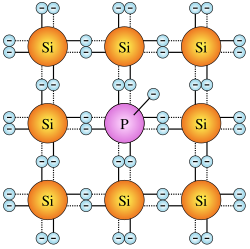
\includegraphics[width=0.42\linewidth]{n-type.png}
  \hspace{0.03\linewidth}
  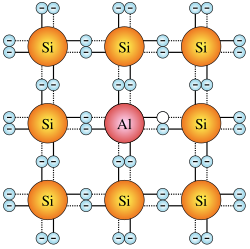
\includegraphics[width=0.42\linewidth]{p-type.png}
  \caption{NMOS 与 PMOS 的最小直觉：前者更适合下拉，后者更适合上拉。这里先抓住“栅控导通”的骨架，器件公式与工艺细节留待后续更专业的课程。}
\end{figure}

把多个 MOS 管组织在一起，就得到所谓上拉网络（pull-up network）和下拉网络（pull-down network）。静态 CMOS 的关键不是“总有电流在跑”，而是尽量让输出稳定地停在高或低两种可判别状态上。因此在正常稳态下，上拉和下拉应当互补工作：要么输出被可靠拉高，要么被可靠拉低，而不是长时间停在中间模糊区。

\subsection{反相器为什么是数字世界的基元}

CMOS 反相器之所以基础，不只是因为它简单，还因为它把数字世界最核心的三个问题压缩进了一个最小对象里。第一，它把输入电平和输出电平之间建立了清楚的因果关系；第二，它让我们第一次可以讨论什么叫高电平、低电平、翻转区和噪声容限；第三，它让“延迟”从抽象名词变成一个具体可观察现象：输出翻转不是瞬时完成的，而是靠负载电容被充电或放电慢慢完成。

\begin{figure}[h]
  \centering
  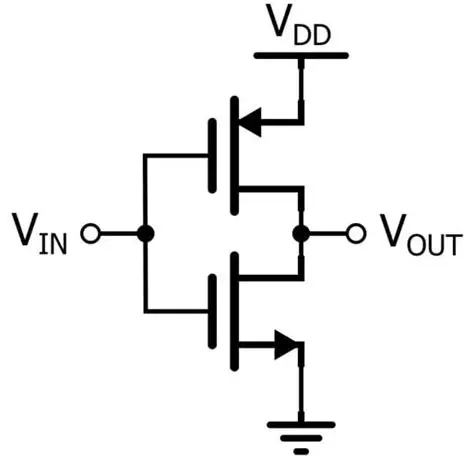
\includegraphics[width=0.55\linewidth]{inverter.png}
  \caption{CMOS 反相器：输入低时 PMOS 导通、输出被上拉；输入高时 NMOS 导通、输出被下拉。逻辑翻转对应的是导通路径翻转。}
\end{figure}

理解反相器时，最值得观察的是“路径”。输入为 0 时，PMOS 打开，\texttt{VDD} 经过上拉路径把输出充到高电平；输入为 1 时，NMOS 打开，输出节点中的电荷通过下拉路径放掉，输出落到低电平。也正因为输出节点带着电容，翻转就会带上真实时间尺度。

\subsection{VTC、噪声容限与门延迟}

电压传输特性（VTC）展示了输入电压连续变化时，输出电压如何响应。它最重要的作用，不是让你背某几个拐点，而是帮助理解为什么逻辑 0/1 能够被可靠地再生出来。曲线两端较平的平台区对应稳定逻辑区，中间陡峭变化区对应门正在翻转的区间。所谓噪声容限，本质上是在问：信号允许带着多大的扰动，后级门仍然能把它重新识别为有效逻辑值。

\begin{figure}[h]
  \centering
  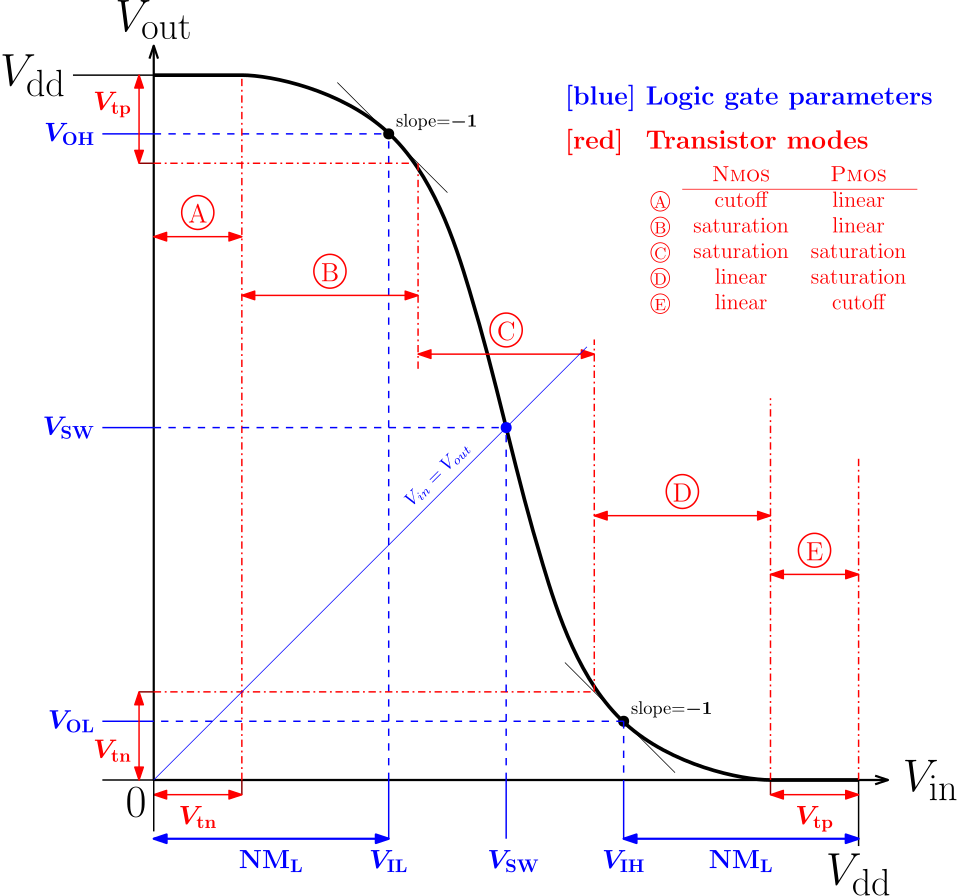
\includegraphics[width=0.56\linewidth]{vtc.png}
  \caption{反相器 VTC 与噪声容限示意。数字抽象依赖的不是“没有噪声”，而是“噪声还不足以把信号推出可判别区间”。}
\end{figure}

与此同时，反相器还让延迟第一次变得具体。输出节点的每次翻转，本质上都是一次电容充电或放电过程；负载越重、扇出越大、输入边沿越慢，翻转往往越慢。输入处于翻转区间时，PMOS 和 NMOS 还可能短时间同时导通，于是出现短路电流。这里最需要建立的工程直觉是：\textbf{门延迟不是一个与环境无关的静态常数，而是会被前后级条件共同塑形的。}

\begin{figure}[h]
  \centering
  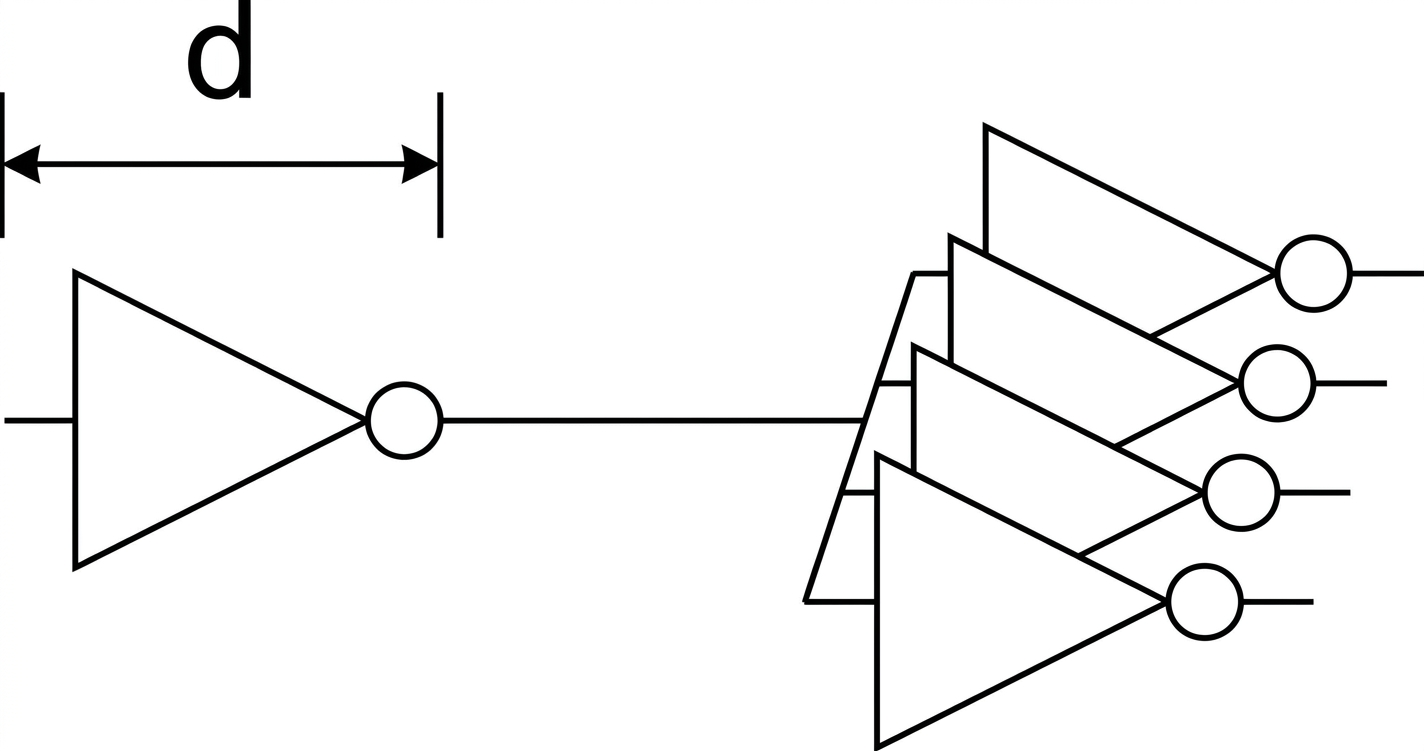
\includegraphics[width=0.46\linewidth]{fo4.png}
  \caption{更重的负载和更大的 fanout 会拉长输出翻转时间。延迟问题从第一个门电路开始就已经存在。}
\end{figure}

\subsection{从反相器到 NAND / NOR}

一旦理解了“上拉 / 下拉网络”这个视角，NAND 和 NOR 的结构就不再像需要死记的图形。NMOS 串联天然更适合表达“多个条件同时满足时才能拉低”的关系，PMOS 并联则天然更适合表达“只要其中一个条件满足就能拉高”的关系。于是，静态 CMOS NAND / NOR 可以看成对布尔关系的一种结构化翻译：不是先写好逻辑，再“硬套”到晶体管图里，而是逻辑关系和导通关系本来就在互相映射。

\begin{figure}[h]
  \centering
  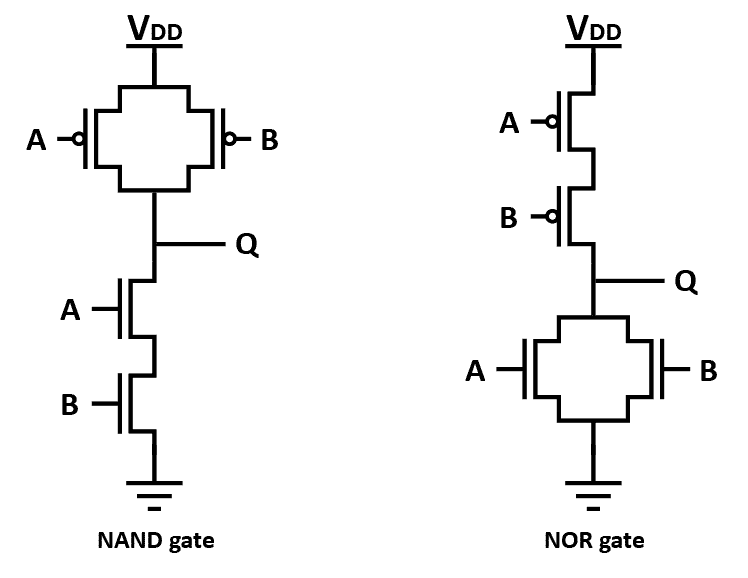
\includegraphics[width=0.76\linewidth]{nand-nor-schema.png}
  \caption{NAND / NOR 的静态 CMOS 结构。晶体管串并关系并不是装饰，而是在实现对应的逻辑条件。}
\end{figure}

这里顺便要把视角再拉回一次物理世界。我们在黑板上画的是门符号和晶体管图，但真实芯片里这些门最终会落成规则化的版图单元，带着明确边界、面积、引脚位置和速度 / 面积权衡。标准单元库中，同一逻辑功能往往会有多个物理变体；本讲不系统展开这些库细节，但至少要让读者知道：逻辑门最后会成为一种有几何形态、有实现成本的对象，而不是永远停留在纸上的符号。

\subsection{组合逻辑与半加器}

组合逻辑的定义很简单：当前输出只依赖当前输入，不依赖过去保存的状态。这个定义看似朴素，却非常重要，因为它把当前这一讲和下一讲的时序逻辑严格区分开来。半加器是这里很合适的收束例子，因为它同时允许我们在真值表、布尔表达式和门级结构之间来回切换。\texttt{SUM} 可以由异或表达，\texttt{CARRY} 可以由与表达；两者都只依赖当前输入 \texttt{A} 和 \texttt{B}，所以它依然是标准的组合逻辑。

\begin{figure}[h]
  \centering
  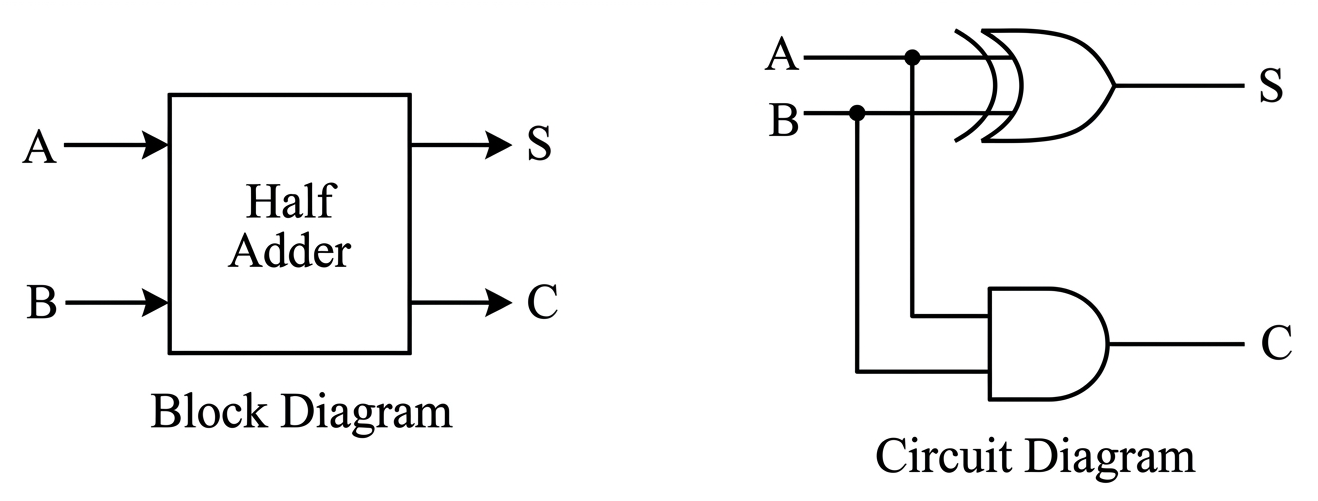
\includegraphics[width=0.54\linewidth]{half_adder.png}
  \caption{半加器把真值表、逻辑表达式与门级结构接到一起，是组合逻辑的典型收束例子。}
\end{figure}

\subsection{竞争、冒险与环形振荡器}

如果此时把“组合逻辑”的定义理解成“没有时间问题”，就会立刻踩坑。逻辑上等价的两条路径，时间上并不一定同时到达；只要不同路径的延迟不同，输出就可能在稳定到最终值之前短暂冒出一个毛刺。这类现象常被称为竞争与冒险。它们提醒我们：逻辑正确与时间上安全不是同一个命题。

\begin{figure}[h]
  \centering
  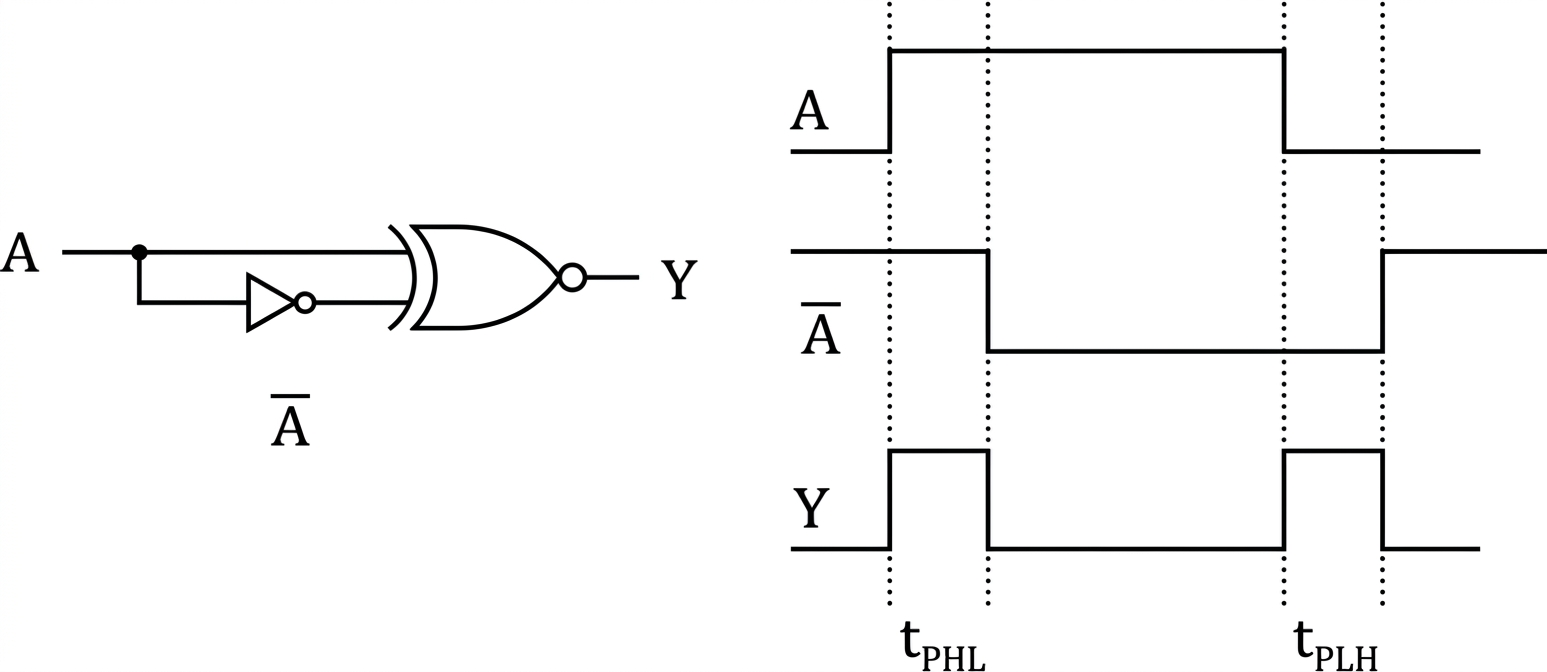
\includegraphics[width=0.60\linewidth]{race_hazard.jpeg}
  \caption{竞争与冒险波形示意。不同路径延迟会让本该“逻辑等价”的网络在瞬时行为上出现毛刺。}
\end{figure}

环形振荡器则把这个提醒再推进一步。奇数个反相器首尾相接后，系统不会收敛到一个稳定值，而会持续振荡。振荡周期直接由每一级延迟决定。如果忽略延迟，就根本解释不了它为什么会振。这也说明：时间不是门电路外部附会上的东西，而是门电路行为本身的一部分。

\section{关键图示或案例}

这一讲最关键的观察方法，不是把所有器件图都背下来，而是学会在不同视角之间切换：器件视角看导通路径，逻辑视角看布尔关系，版图视角看最终落地的物理对象，波形视角看这些结构在时间上如何表现。只要能在这四个视角之间来回走动，后面的 RTL、综合、时序分析就不会再像彼此割裂的几门课。

\begin{tipbox}
这一讲先抓住三件事就够了：第一，逻辑门是在组织导通路径；第二，反相器是最小完整基元；第三，组合逻辑虽然没有“状态”，但已经有“时间”。后面的标准单元库、时序分析、逻辑优化都会沿着这三条线继续加深。
\end{tipbox}

\begin{warnbox}
不要把“组合逻辑”误解成“没有延迟、没有风险、只看真值表就够了”。真值表只刻画稳态逻辑关系，不负责保证不同路径在时间上同时到达，更不负责处理毛刺被后级错误采样的后果。
\end{warnbox}

\section{本讲小结}

本讲真正建立的，不是一张更长的逻辑门清单，而是一条从物理世界通向逻辑世界的因果链：MOS 管像受控开关，因此可以组成互补的上拉 / 下拉网络；互补网络让反相器和基础逻辑门成为稳定可实现的对象；逻辑门进一步组织成组合逻辑网络；而延迟、负载和路径差异又让时间问题从第一讲起就已经存在。这样一来，下一讲引入寄存器、时钟、setup/hold 和 metastability 时，读者看到的不再是一组突然冒出来的新术语，而是同一条链在时间维度上的继续展开。

\section{练习题}

\begin{enumerate}
  \item 画出 CMOS 反相器，并分别说明输入为 0 与输入为 1 时，哪一条导通路径在工作、输出为什么会得到对应的逻辑值。
  \item 对照 NAND / NOR 的静态 CMOS 结构图，解释 NMOS 串联 / 并联与 PMOS 串联 / 并联分别在表达怎样的逻辑条件。
  \item 写出半加器的真值表，并根据真值表推导 \texttt{SUM} 和 \texttt{CARRY} 的逻辑表达式，再画出对应门级结构。
  \item 给出一个两条路径延迟不同的组合逻辑例子，解释为什么输出会出现毛刺；进一步讨论，在什么情况下这个毛刺可能会真正造成系统错误。
\end{enumerate}

\end{document}
